\documentclass[letterpaper,10pt]{article}

\usepackage{titling}
\usepackage{listings}
\usepackage{url}
\usepackage{setspace}
\usepackage{subfig}
\usepackage{sectsty}
\usepackage{pdfpages}
\usepackage{colortbl}
\usepackage{multirow}
\usepackage{relsize}
\usepackage{amsmath}
\usepackage{fancyvrb}
\usepackage{amsmath,amssymb,amsthm,graphicx,xspace}
\usepackage[titlenotnumbered,noend,noline]{algorithm2e}
\usepackage[compact]{titlesec}
\usepackage{paratype} 
\usepackage[T1]{fontenc}
\usepackage{tikz}
\usetikzlibrary{arrows,automata,shapes,trees,matrix,chains,scopes,positioning,calc}
\tikzstyle{block} = [rectangle, draw, fill=blue!20, 
    text width=2.5em, text centered, rounded corners, minimum height=2em]
\tikzstyle{bw} = [rectangle, draw, fill=blue!20, 
    text width=4em, text centered, rounded corners, minimum height=2em]

\definecolor{namerow}{cmyk}{.40,.40,.40,.40}
\definecolor{namecol}{cmyk}{.40,.40,.40,.40}

\let\LaTeXtitle\title
\renewcommand{\title}[1]{\LaTeXtitle{\textsf{#1}}}


\newcommand{\handout}[5]{
  \noindent
  \begin{center}
  \framebox{
    \vbox{
      \hbox to 5.78in { {\bf ECE254: Operating Systems and Systems Programming } \hfill #2 }
      \vspace{4mm}
      \hbox to 5.78in { {\Large \hfill #4  \hfill} }
      \vspace{2mm}
      \hbox to 5.78in { {\em #3 \hfill} }
    }
  }
  \end{center}
  \vspace*{4mm}
}

\newcommand{\lecture}[3]{\handout{#1}{#2}{#3}{Lecture #1}}
\newcommand{\tuple}[1]{\ensuremath{\left\langle #1 \right\rangle}\xspace}

\addtolength{\oddsidemargin}{-1.000in}
\addtolength{\evensidemargin}{-0.500in}
\addtolength{\textwidth}{2.0in}
\addtolength{\topmargin}{-1.000in}
\addtolength{\textheight}{1.75in}
\addtolength{\parskip}{\baselineskip}
\setlength{\parindent}{0in}
\renewcommand{\baselinestretch}{1.5}
\newcommand{\term}{Spring 2015}

\singlespace


\begin{document}

\lecture{ 26 --- Scheduling Algorithms }{\term}{Jeff Zarnett}

\section*{Scheduling Algorithms}

Earlier we saw one example of a simple scheduling algorithm: always choose the highest priority (non-blocked) task, and execute it. There are many other choices we could make. We will examine the following options:
\begin{enumerate}
	\item Highest Priority, Period
	\item First-Come, First-Served
	\item Round Robin
	\item Shortest Process Next
	\item Shortest Job First
	\item Smallest Remaining Time
	\item Highest Response Ratio Next
	\item Multilevel Queue (Feedback)
	\item Guaranteed Scheduling
	\item Lottery
\end{enumerate}

The OS may maintain data about each process to be used in making decisions about scheduling~\cite{osi}:

\begin{enumerate}
	\item The time spent waiting to run.
	\item The time spent executing.
	\item The total time of execution.
\end{enumerate}

The first two criteria in the list can easily be measured, but the third one must be estimated or supplied by the user. Old batch systems did sometimes ask users to provide an estimate of how long they thought a task was likely to take. If the user underestimated, then execution would be halted at the time they said, even if his or her operation was unfinished. But the higher the estimate, the lower the priority the task received; if too high the user task might never be scheduled to run at all. Operating systems do not ask the users in desktop systems to estimate how long a process will run, but supercomputers and other batch jobs may still consider this as a criterion.

\subsection*{Highest Priority, Period}

Implementing this is not difficult; we could have some priority queues (one for each priority level). If a task is not blocked, put it in its appropriate priority queue. If the process's priority is changed (manually or otherwise), move it to its new home. We might have a priority heap, or just one big linked list or array that we keep sorted by priority. Many options.

The flaw in this has already been identified: it is vulnerable to starvation. A process of relatively low priority may never get the chance to run, because there is always something better to do right now. Humans presumably encounter situations like this all the time. Software projects may have bug reports open for years on end because they are never important enough to be addressed. In my personal life, there are books I'd like to read (the example ``Der Deutsch-Franz\"osische Krieg 1870/71'' springs to mind), but I never get to them because something else always comes up... work to do, another book to read, a social event...

In some systems this is a desirable property. It does not fulfill all short term scheduling criteria, notably response time and fairness. It may be suitable for life-and-safety-critical systems, such as the process to control a robot arm, to prevent a situation where the robot arm goes through the wall and the building falls down and you're dead.

\subsection*{First-Come, First-Served}
This is an obvious algorithm that is simple to implement. Whichever process requests the CPU first gets the CPU first. Just imagine a queue of processes in which all processes are equal. A process enters the queue at the back and whichever process is at the front will be dequeued and get to run.  If the current process finishes or is blocked for some reason, the next ready process is selected. This is actually a simplification of the highest priority, period scheme, because it ignores priority altogether. All processes will get a chance to run eventually, so low priority processes will not starve.

FCFS can result in some undesirable outcomes. The average waiting time for processes might vary wildly. Consider if we have three processes, $P_{1}$, $P_{2}$, and $P_{3}$. Let us say that $P_{1}$ needs 24 units of CPU time; $P_{2}$ and $P_{3}$ require 3 units each.

\begin{center}
	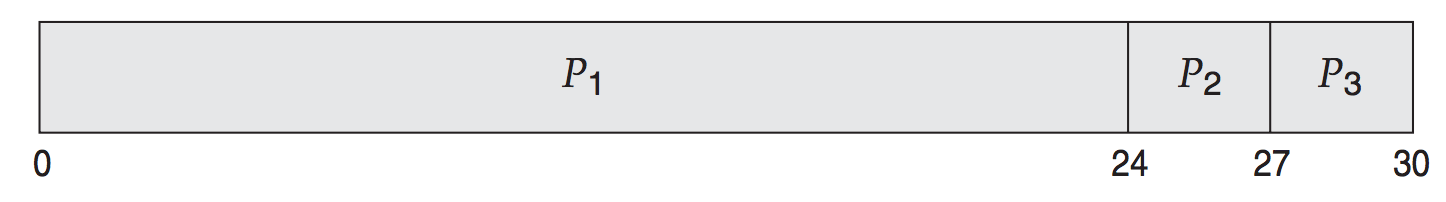
\includegraphics[width=0.7\textwidth]{images/fcfs-1.png}\\
	First-Come, First-Served Scheduling for $P_{1}$, $P_{2}$, and $P_{3}$~\cite{osc}.
\end{center}

The total time needed to complete all processes is 30 units. The average completion time, however, is $(24 + 27 + 30) / 3$ = 27 units. Nothing wrong with this. Suppose, however, the processes arrived in a slightly different order:

\begin{center}
	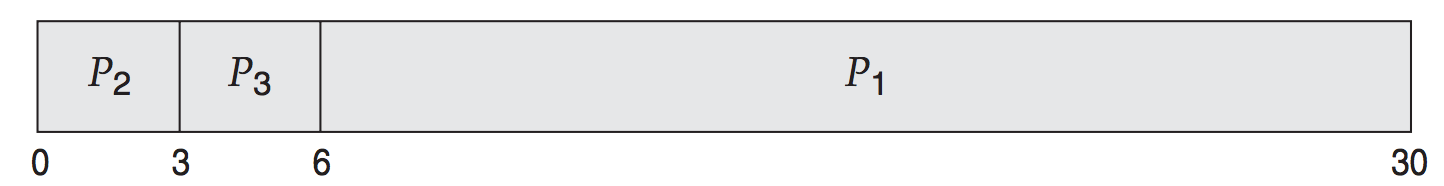
\includegraphics[width=0.7\textwidth]{images/fcfs-2.png}\\
	$P_{1}$, $P_{2}$, and $P_{3}$ arriving in a different order~\cite{osc}.
\end{center}

If $P_{1}$ arrived last instead, then the picture is somewhat different. It still takes 30 units of time to complete all processes, but the average completion time is $(3 + 6 + 30) / 3)$ = 13 units. Now this might make a big difference to the user: seeing processes 2 and 3 completed sooner will probably be viewed positively. Still, we consider it an undesirable thing that we have such a dramatic difference in how long $P_{2}$'s turnaround time is.

FCFS as a scheduling algorithm also tends to favour CPU-Bound processes rather than I/O-Bound processes. When a CPU-Bound process is running, the I/O bound processes must wait in the queue like everybody else. This might lead to inefficient use of the resources; disk is slow so we would like to keep it busy at all times. If a disk write is completed and there is a process that would like to read something from disk, it would be ideal to issue that read straight away so the disk is constantly in use. With FCFS, however, the I/O devices are likely to suffer idle periods~\cite{osi}.

The FCFS algorithm as it is generally described, is non-preemptive; a process that gets selected from the front of the queue runs until there is a reason to make the swap. So in theory, one process could monopolize the CPU (remember that some people are jerks). If we modify FCFS with periodic preemption, then we get a new system, Round Robin.

\subsection*{Round Robin}
The idea of time slicing has already been introduced: every $t$ units of time, a timer generates an interrupt that is the prompt to run the short-term scheduler. Time slicing itself can be combined with many of the strategies for choosing the next process, but when it is combined with FCFC we get Round Robin. 

The principal issue is: how big should $t$ be? If $t$ is too long, then processes may seem to be unresponsive while some other process has the CPU, or short processes may have to wait quite a while for their turn. If $t$ is too short, the system spends a lot of time handling the clock interrupt and running the scheduling algorithm and not a lot of time actually executing the processes~\cite{osi}.

On the principle of ``don't guess; measure'' we could make a decision about the size of $t$ based on the patterns of the system. If we know that the typical process tends to run for $r$ units of time before getting blocked on I/O or something, then it would be logical to choose $t$ such that it is slightly larger than $r$. If $t$ is smaller than $r$, then processes will frequently be interrupted by the time slice. Processes that are going to use a lot of CPU will be split up over multiple time slices anyways, but it's frustrating if the process would take 1.1 time slices. If $t$ is larger than $r$, many processes will not run up against that time slice limit and will hopefully accomplish a useful chunk of work before getting blocked for I/O or some other reason. 

Thinking about this further, Round Robin tends to favour CPU-Bound processes. An I/O-Bound process spends a lot less time using the CPU. It runs for a short time, gets blocked on I/O, then when the I/O is finished, it goes back in the ready queue. So CPU-Bound processes are getting more of the CPU time.

Round Robin can be improved to Virtual Round Robin to address this unfairness. It works like Round Robin, but a process that gets unblocked after I/O gets higher priority. Instead of just rejoining the general queue, there is an auxiliary queue for processes that were previously blocked on I/O. When the scheduler is choosing a process to run, it takes them from the auxiliary queue if possible. If a process simply ran up against the time limit, it goes into the regular ready queue instead. If dispatched from the auxiliary queue, it runs for up to the as-yet-unused fraction of a slice~\cite{vrr}.

\begin{center}
	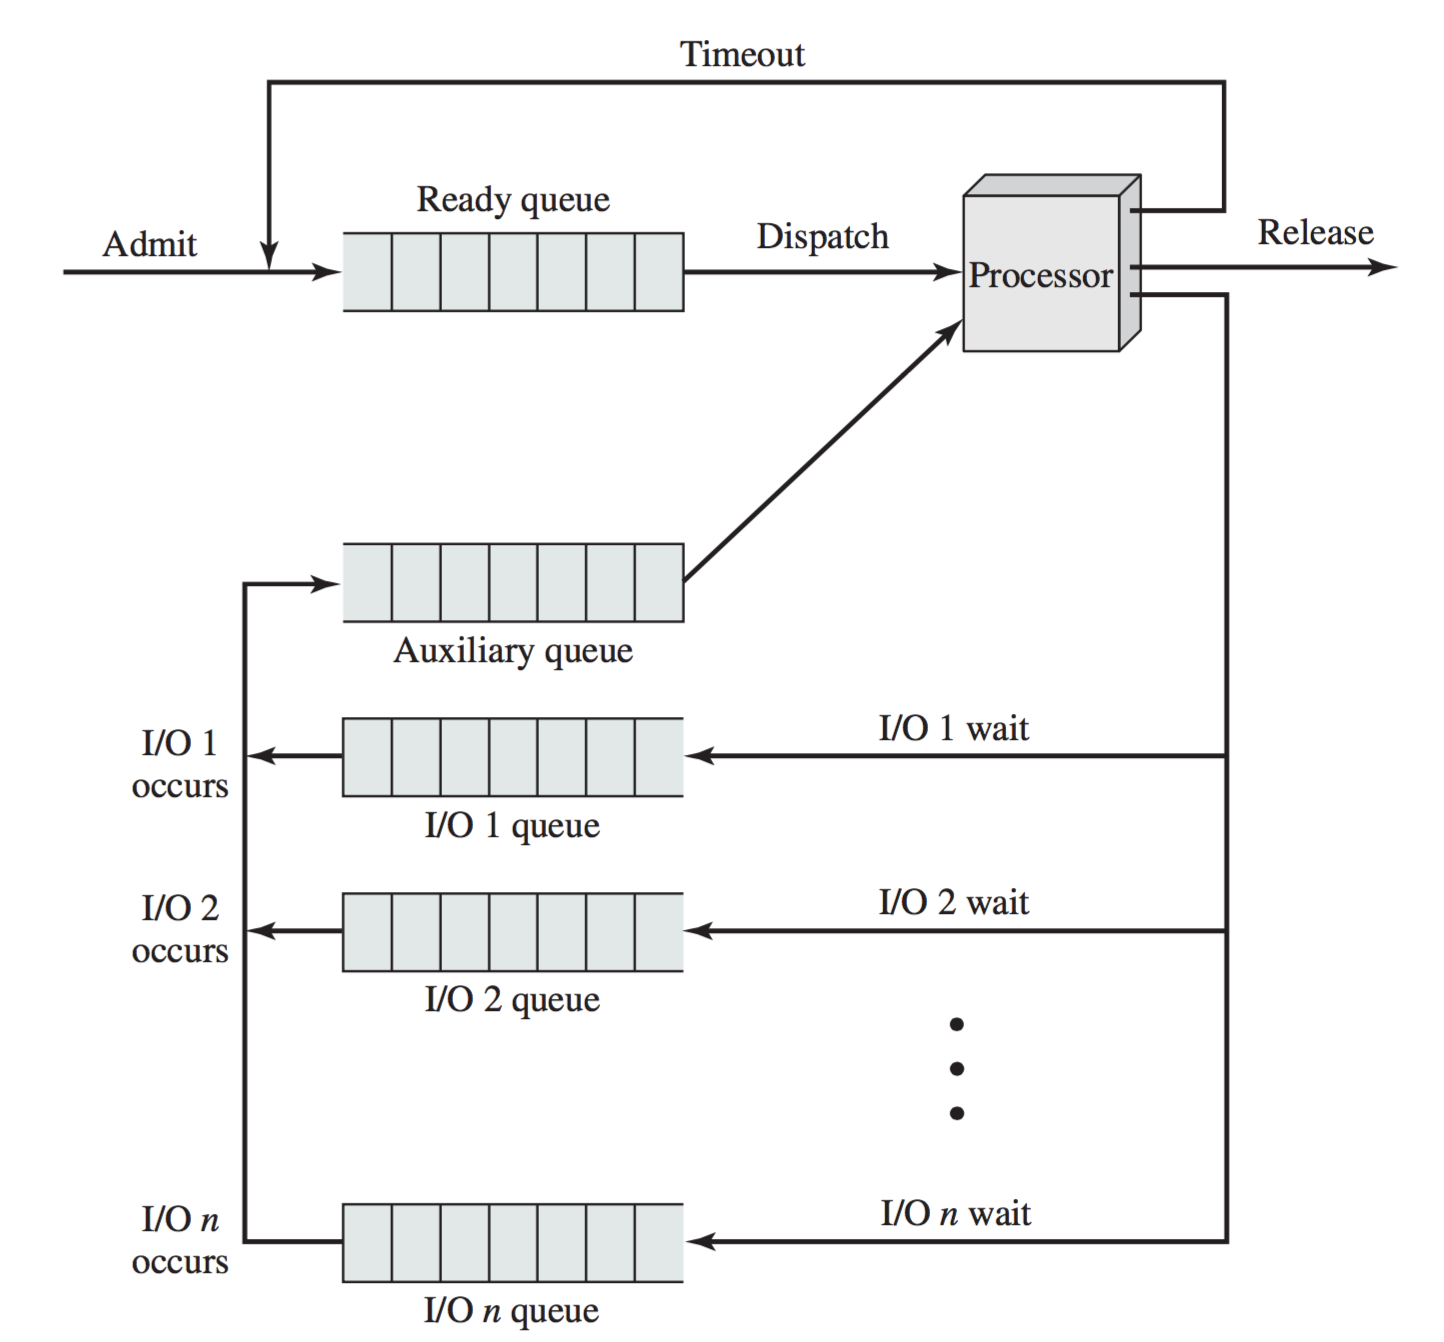
\includegraphics[width=0.65\textwidth]{images/virtual-round-robin.png}\\
	Queueing diagram for the Virtual Round Robin scheduling approach~\cite{osi}.
\end{center}

\subsection*{Shortest Process Next}
If some information is available about the total length of execution then we may wish to give priority to short processes. We let short processes go first to get them over with quickly. The reason is made clear by the second example of FCFS from earlier; though it still took 30 units of time, total, the average time to completion of a task was a lot lower when the shorter processes of $P_{2}$ and $P_{3}$ ran before $P_{1}$. This means we will get faster turnaround times and better responsiveness, but longer processes may be waiting an unpredictable amount of time.

This is the sort of thing that used to happen in batch job processing on mainframes. The programmer was asked to give an estimate of the amount of time the program (e.g., compile) would run. If the programmer's estimate was too low, the program execution would be terminated early. If the programmer's estimate was too high, the job may never be scheduled to run, or at least, have to wait a very long time. 

This might work, but you have noticed that the OS does not ask you, when you start a text editor, roughly how long you expect to be. Your boss on co-op may not be so accommodating. This is also a global assessment: how long the whole process takes. It might be better to worry about the length of CPU bursts and make decisions somewhat more locally...

\subsection*{Shortest Job First}
This strategy, unfortunately, is not given quite the right name, but it's the common name for the scheme. We should call it ``shortest next CPU burst'', but then again, the other sciences are not so good at naming things either... the Red Panda is not a Panda at all.

Right, naming aside, the goal is to choose the process that is likely to have the smallest CPU burst. If two are the same, then FCFS can break the tie (or just choose randomly).  If we have 4 processes, $P_{1}$ through $P_{4}$, whose predicted burst times are 6, 8, 7, and 3 respectively, we should schedule then such that the order would be $P_{4}, P_{1}, P_{3}, P_{2}$:

\begin{center}
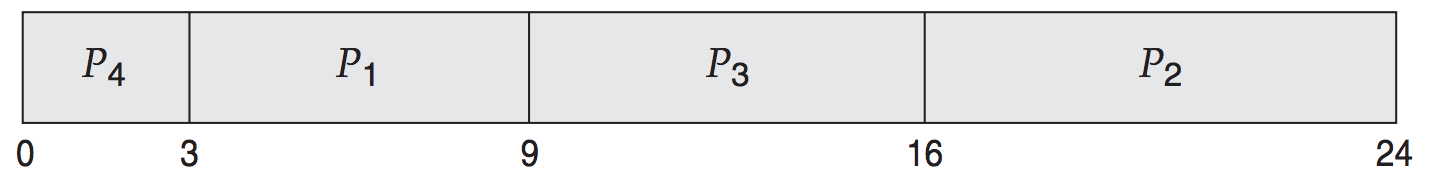
\includegraphics[width=0.7\textwidth]{images/sjf.png}\\
Scheduling the jobs with the shortest CPU burst first~\cite{osc}.
\end{center}

The average waiting time is $(3 + 16 + 9 + 0) / 4$ = 7 units of time. This is significantly better than the FCFS scheduling. In fact, the algorithm is provably optimal in giving the minimum average waiting time for processes. Moving a short process up means it finishes faster, and that decreases its waiting time, while moving longer processes back increases their waiting time. Overall, this scheme is a net positive because the decreases outweigh the increases~\cite{osc}.

The problem is predicting the CPU burst times. The best thing we may be able to do is gather information about the past and use that to guess about the future. The formula in~\cite{osi}:

\begin{center}
$S_{n+1} = \frac{1}{n}\displaystyle\sum_{i=1}^{n}T_{i}$
\end{center}

where: $T_{i}$ is the burst time for the $i$th instance of this process; $S_{i}$ is the predicted value for the $i$th instance; and $S_{1}$ is a guess at the first value (not predicted, because we have no data to go on at that point). Instead of picturing it as a sum each time, we can modify the equation to just update the value:

\begin{center}
$S_{n+1} = \frac{1}{n}T_{n} + \frac{n - 1}{n} S_{n}$
\end{center}

This routine, as you may have guessed, gives each term in the summation equal weight of $\frac{1}{n}$. What we would like to do is give greater weight to the more recent values. The strategy for doing so, as in~\cite{osi} is exponential averaging. We define a weighting factor $\alpha$, somewhere between 0 and 1, that determines how much weight the observations are given:

\begin{center}
$S_{n+1} = \alpha T_{n} + (1 - \alpha) S_{n}$
\end{center}

Thus, the older the observation, the less it is counted in the average. The larger the value of $\alpha$, the more the recent observations matter. The diagram below compares simple averaging (no use of $\alpha$ to age the data) against the values of $\alpha$ of 0.8 and 0.5. The case of $\alpha = 0.8$ assigns significantly more weight to the most recent 4 events than the others.

\begin{center}
	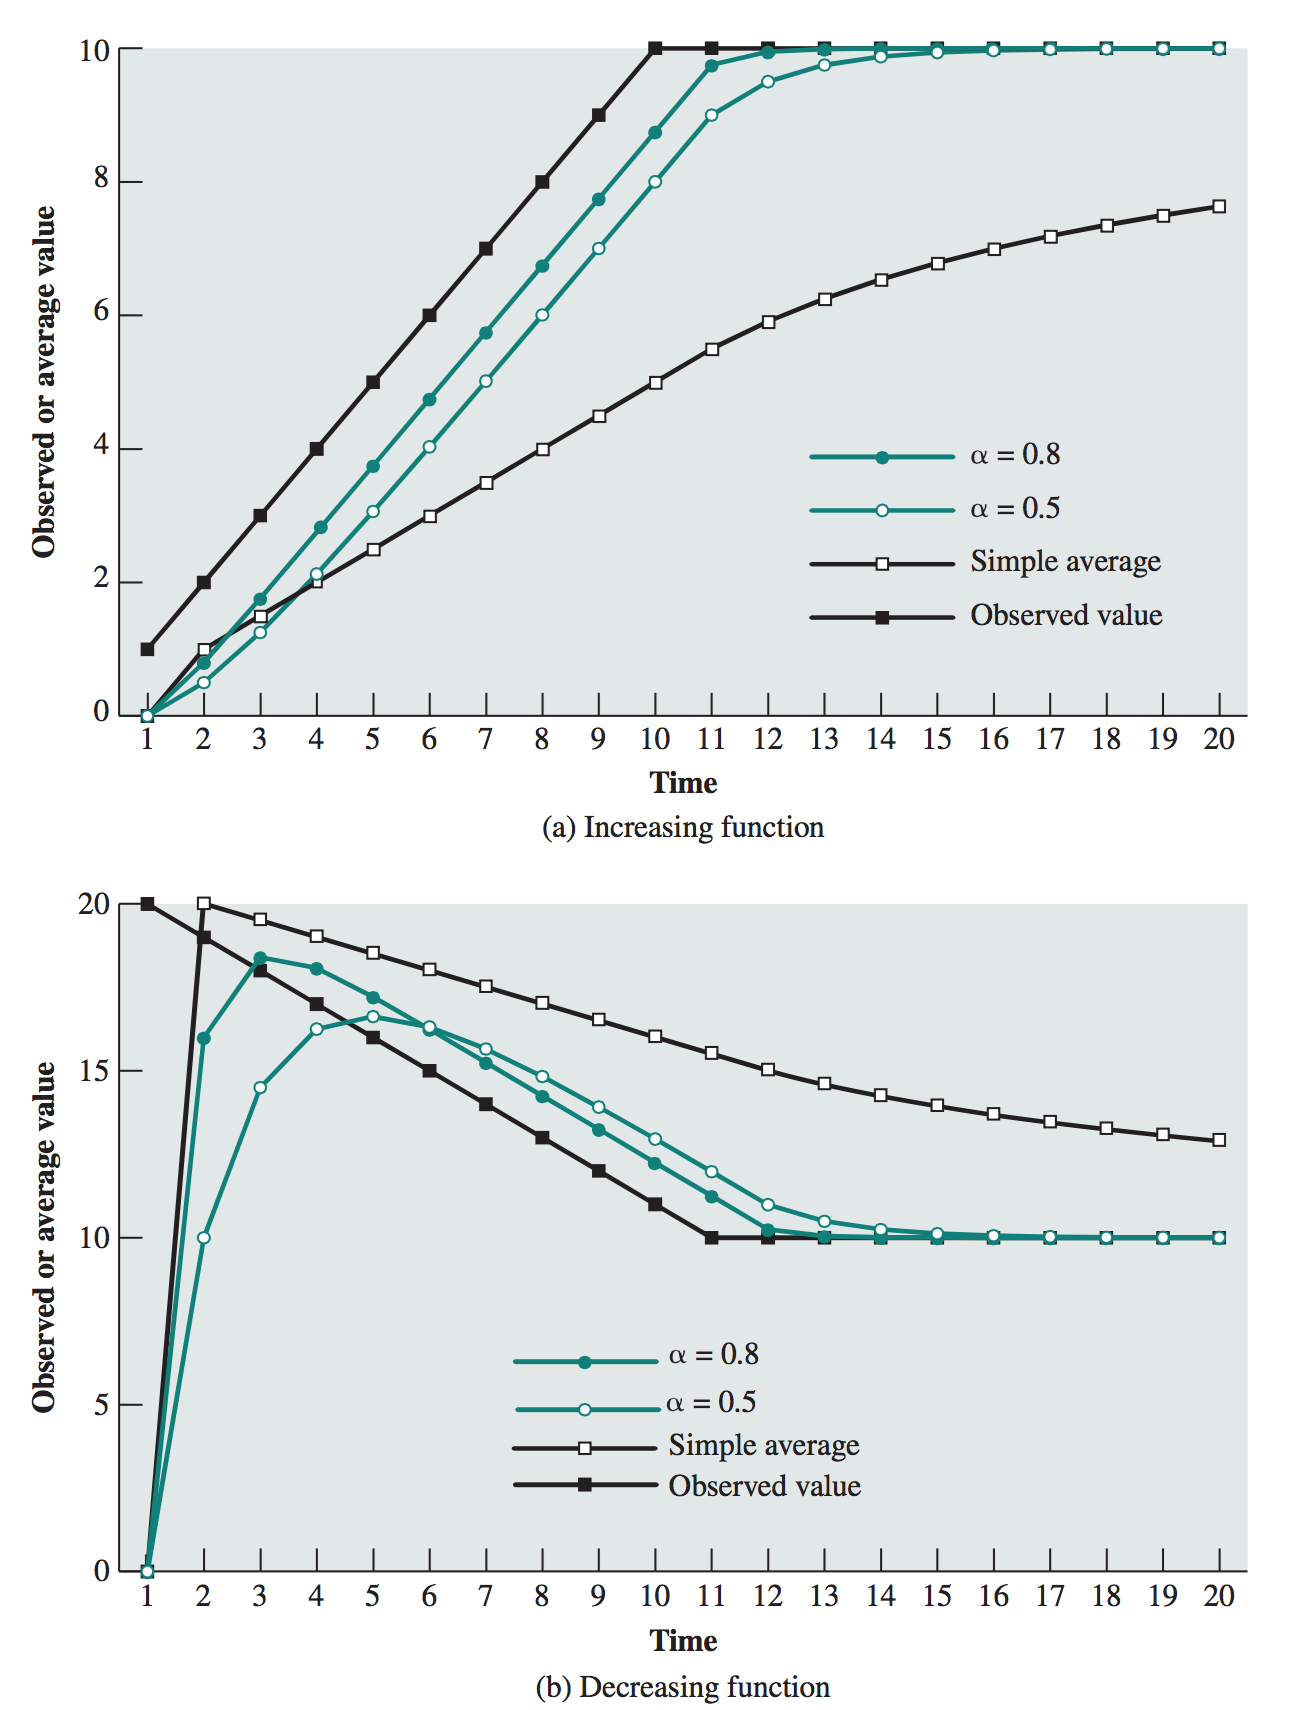
\includegraphics[width=0.7\textwidth]{images/exponential-averaging.png}\\
	Use of Exponential Averaging~\cite{osi}.
\end{center}


We might give an estimate of $S_{1} = 0$ to start with, which gives new processes priority and a chance to get started. After they have started and run a bit, we will have some data. But first we have to give them a chance.

\begin{center}
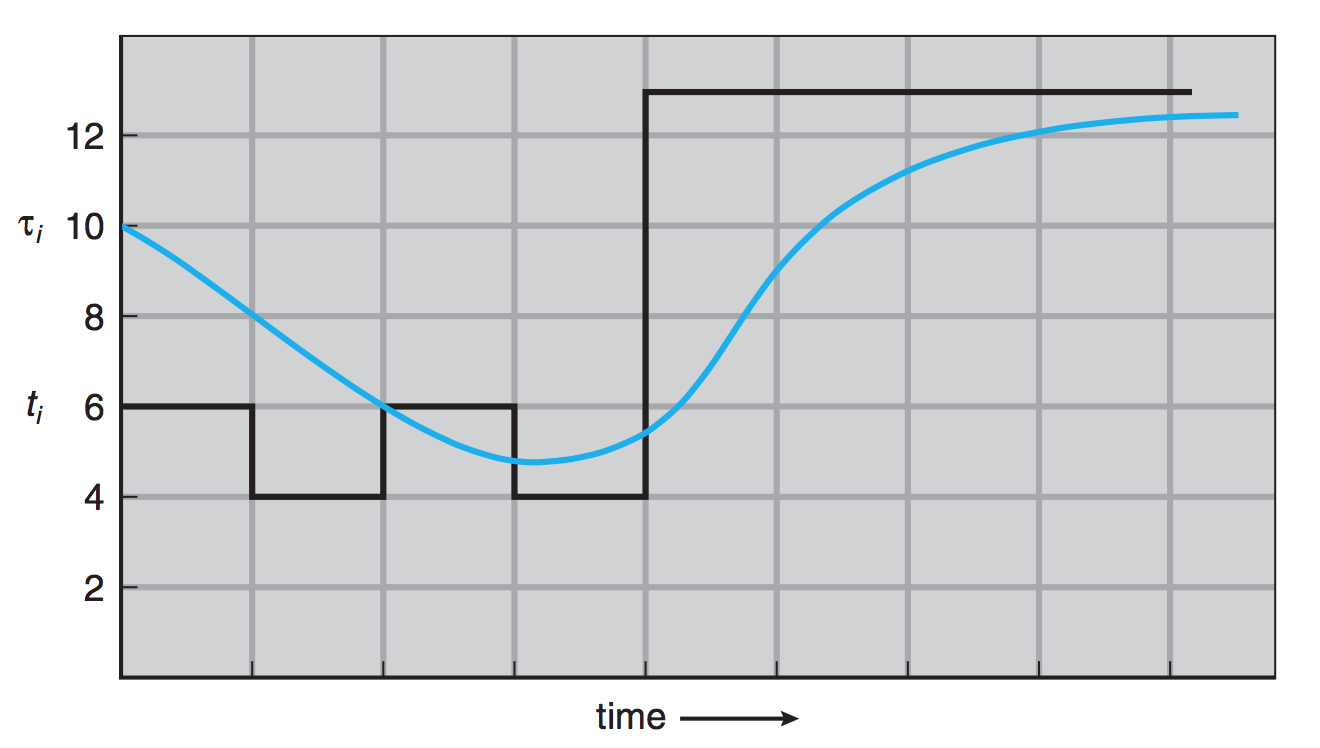
\includegraphics[width=0.7\textwidth]{images/sjf-2.png}\\
Predictions ($\tau_{i}$) and actual CPU burst ($t_{i}$) example~\cite{osc}.
\end{center}

There is still a chance that longer processes will starve; if there is a constant stream of shorter processes, they will continue to get scheduled ahead of a long one, causing the long one to wait unreasonably long...

\subsection*{Shortest Remaining Time}

Shortest remaining time is a modification of the preceding strategy, which allows for some additional preemption. When a new process is scheduled or an old one becomes unblocked, the scheduler will evaluate if it has a shorter predicted running time than the currently-executing process. If so, then the new (or unblocked) process will displace the currently-executing one and start running right away.

As with Shortest Job First, there is a chance that long processes will starve because of a steady stream of shorter processes. If we choose $S_{1}$ to be zero for new processes, it means they will always preempt the running process. This may or may not be desirable.

One advantage we have in choosing SRT is that it means we no longer need to have time slicing. Instead of interrupting the running process every $t$ units of time, the other interrupts (users launching programs, hardware operations completed, etc) will be the prompts to run the scheduler. Thus, the system does not spend any time handling the clock interrupts, which will be a performance increase. Handling the clock interrupt is not expensive, but even an inexpensive operation, done a million times, will eventually add up...~\cite{osi}

\subsection*{Batch and Interactive}

So far the scheduling routines we have looked at are more suitable to batch processing systems (mainframes, supercomputers, etc.) than to interactive desktop systems. The remaining scheduling algorithms in the list will look a lot more like what we expect to see on our laptops and phones...

\bibliographystyle{alpha}
\bibliography{254}


\end{document}